%% ----------------------------------------------------------------
%% Thesis.tex -- MAIN FILE (the one that you compile with LaTeX)
%% ---------------------------------------------------------------- 

% Set up the document
\documentclass[a4paper, 11pt, oneside]{Thesis}  % Use the "Thesis" style, based on the ECS Thesis style by Steve Gunn
\graphicspath{{Figures/}}  % Location of the graphics files (set up for graphics to be in PDF format)

% Include any extra LaTeX packages required
\usepackage{verbatim}  % Needed for the "comment" environment to make LaTeX comments
\usepackage{vector}  % Allows "\bvec{}" and "\buvec{}" for "blackboard" style bold vectors in maths
\hypersetup{urlcolor=blue, colorlinks=true}  % Colours hyperlinks in blue, but this can be distracting if there are many links.

%% ----------------------------------------------------------------
\begin{document}


\clearpage  % End of the Acknowledgements
%% ----------------------------------------------------------------

\pagestyle{fancy}  %The page style headers have been "empty" all this time, now use the "fancy" headers as defined before to bring them back


%% ----------------------------------------------------------------
\lhead{\emph{Contents}}  % Set the left side page header to "Contents"
\tableofcontents  % Write out the Table of Contents

%% ----------------------------------------------------------------
\lhead{\emph{List of Figures}}  % Set the left side page header to "List if Figures"
\listoffigures  % Write out the List of Figures



%% ----------------------------------------------------------------
\clearpage  % Start a new pageFlrc



%% ----------------------------------------------------------------
\mainmatter	  % Begin normal, numeric (1,2,3...) page numbering
\pagestyle{fancy}  % Return the page headers back to the "fancy" style

% Include the chapters of the thesis, as separate files
% Just uncomment the lines as you write the chapters
\lhead{\emph{Chapter 1}}
\chapter{Introduction}
\section{Background}
Flash systems are gaining their presence everywhere from mobile devices to servers with RAID and SAN architectures. SSD has become more popular due to their high speed, low noise, low power consumption and reliability. 

There are many reasons for flash storage picking up in the storage industry. 
\textbf{\textit{The main advantages of NAND flash are: }}
\begin{enumerate}

\item Better performance capabilities, speed in particular. Flash storage can get the system up and running in few seconds. Enterprises that need fast processing of their business applications and retrieve/store data quickly prefer flash storage systems. 

\item The durability is very high compared to hard drives which have mechanical parts like the spinning disks, head etc. The chances of losing data due to equipment mishandling is low. This feature is very important for the business who are more concerned about the security of their data. The absence of mechanical moving parts also contributes to higher performance. 

\item They consume very less power, thereby reducing the energy costs greatly.

\end{enumerate}
There are a few disadvantages of the flash system as well and \textbf{the main disadvantage which is of interest to us is the endurance.} 

\textbf{\textit{Endurance}} is just a fancy name for \textbf{\textit{life time}} of the storage systems. Endurance of a storage system is a very important aspect as it directly correlates to the lifetime of data. Compared to the hard drives, the NAND flash has a very low endurance. They have a finite program-erase cycles because of the process involved in the program erase operations for every write. \textbf{\textit{NAND flash uses two methodologies to write data: }} 
\begin{enumerate}

\item  Quantum Tunneling.
\item  Hot Electron Injection.
\end{enumerate}

Each write to these systems causes physical damage due to the above mechanisms. Refer figure \ref{fig:1} for quantum tunneling and refer figure \ref{fig:2} for hot electron injection method. The damages are due to the high heat generated. The oxide layer in the flash systems which are used to trap the charges is degraded every time a write is performed. The charge stored representing either a 0 or 1 cannot be differentiated due to the damage and hence the flash systems become unusable after this point. The damage eventually piles up to decrease the endurance time of the flash system. The other disadvantage of the flash systems compared to the hard drives is the cost per GB. NAND flash is much more expensive than the hard drives. The price of flash storage is gradually decreasing but currently SSD are more expensive.

\begin{figure}[h]
    \centering
    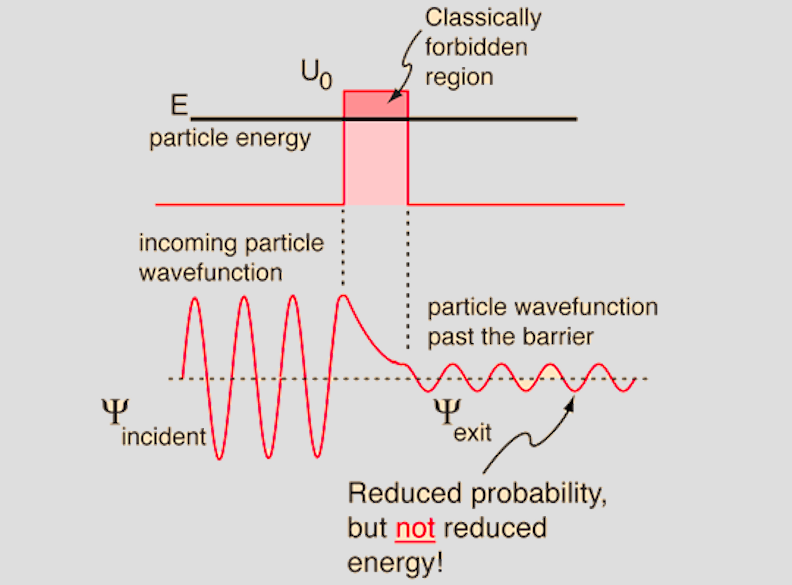
\includegraphics[width=\textwidth]{quantum}
    \caption{Quantum Tunneling \textsuperscript{[12]}}
    \label{fig:1}
\end{figure}

\begin{figure}[h]
    \centering
    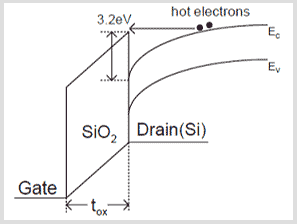
\includegraphics[width=\textwidth]{hot_electrons}
    \caption{Hot Electrons Injection\textsuperscript{[13]}}
    \label{fig:2}
\end{figure}
There are many distributed system applications which require a balance out between strong and eventual consistency. For example, consider an online shopping website. Use case such as the billing process should be strongly consistent whereas a recommendation window, based on the users` browsing history can be weakly consistent. For such systems, the proposed solution can be deployed for use cases which do not need strong consistency.

\section{Motivation}
When we consider the flash storage, we know that the number of writes which can be performed on flash storage is in the range of \textbf{$10^\textsuperscript{5}$ - $10^\textsuperscript{7}$}.
Due to the design of the flash memory, we cannot perform in-place update on a block of data. So we have to go through an erase of the block which completely erases the page by making all bits to zero (by having negative charge) and then perform the write cycle. But this leads to a condition called uneven wearing because a part of the storage is accessed rarely where the data is used only for reading (say a copy of the movie image) and the other part of the data is accessed often for writing (say a part of the disk which is used for paging). To solve this problem \textbf{“Wear Leveling”} was introduced.
 
 \textit{But wear leveling increases the number of writes in a flash storage} i.e. the \textbf{write amplification.}
 
 \textbf{\textit{The main idea of this research is to reduce the number of writes if the same piece of data is present in the RAM or in the storage replica which is about to change shortly.}}

\section{Development Environment}

The project was mainly developed in University of California Santa Cruz under the guidance of Professor Jishen Zhao in her lab. 

Initially it was proposed to develop the code in C language to support and run on Unix based Operating System running any data base. Later for simplicity and to increase the rate of development to implement the proof of concept it was decided to use Python language and pickel DB.

 Apart from the pickle DB package for this project we have used python packages like matplotlib, tox, socket and pytest which will be discussed in detail later.

For executing the program, we required minimum 2 separate computers to test the code.  Later moved to virtual environment by using the "Oracle virtual box" for dvelopment and test. The code has been tested on different operating systems like the MAC OS, Windows and Linux setup which were used both as a client and server configurations. More details about the architecture and system design is explanined later in the implementation section. 

%I have started the project from the scratch and uploaded my code under my git repository:  "https://github.com/Narendrakumarg1728/write_reduction_in_Distributed_replicas"

\textsuperscript{[1]} For the project we have used the python version 2.7. Install python version 2.7 by running the below commands on different Operating systems or can also be installed using Anaconda .


1. Ubuntu.

sudo apt-get install build-essential checkinstall
sudo apt-get install libreadline-gplv2-dev libncursesw5-dev libssl-dev libsqlite3-dev tk-dev libgdbm-dev libc6-dev libbz2-dev
cd ~/Downloads/
wget https://www.python.org/ftp/python/2.7.12/Python-2.7.12.tgz
tar -xvf Python-2.7.12.tgz
cd Python-2.7.12
./configure
make
sudo checkinstall

2. MAC OS.

Download package from "https://www.python.org/downloads/mac-osx/" then double click to install python.

3. Windows OS.

Download package from "https://www.python.org/downloads/windows/" then double click to install python. 


In order to test if the development environment is working as expected, type ``python -v". The versions of all the packages and the python version is displayed along with the python interpreter prompt at the end as shown in the figure \ref{fig:3}.

\begin{figure}[h]
    \centering
    \includegraphics[width=\textwidth]{python}
    \caption{Python version}
    \label{fig:3}
\end{figure}


\subsection{TOX}
Tox is a tool that creates a virtual environment for python. It is very helpful for creating a separate virtual environment for our development and testing.  Use the command "pip install tox" to install tox and then run the command "tox-quickstart" for setting up the environment as shown in the below figure \ref{fig:4}.

\begin{figure}[h]
    \centering
    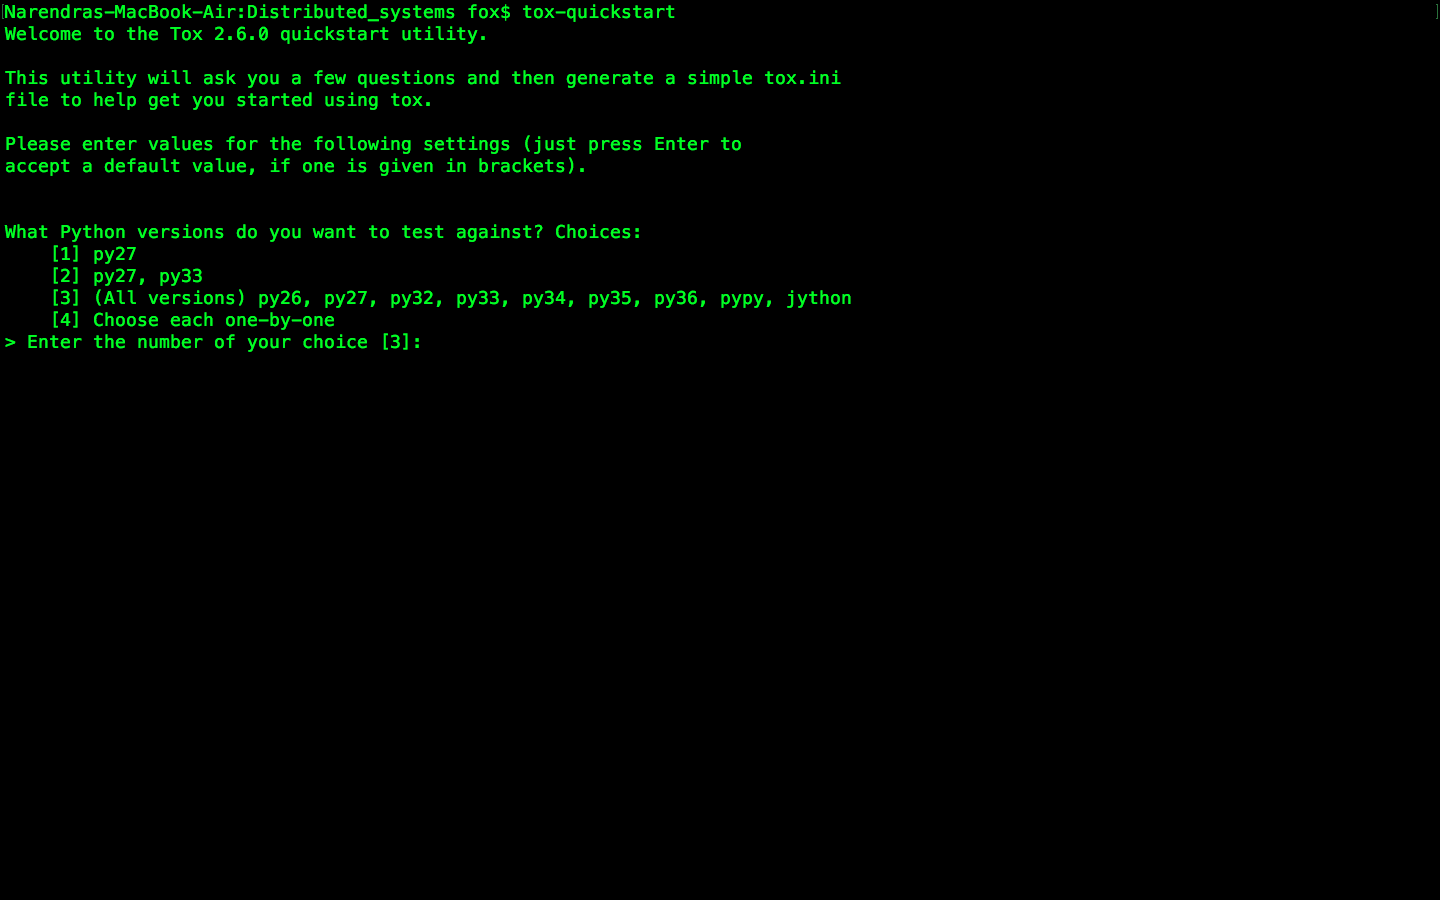
\includegraphics[width=\textwidth]{tox}
    \caption{tox-quickstart}
    \label{fig:4}
\end{figure}

\subsection{PYTEST}

For testing and debugging of the python code we have used the python test frame work pytest. To install pytest use the command "pip install pytest" then for debugging using pytest use the inbuilt function "assert" which will be discussed later in detail. To test and debug run the command pytest as shown in the figure \ref{fig:5}.

\begin{figure}[h]
    \centering
    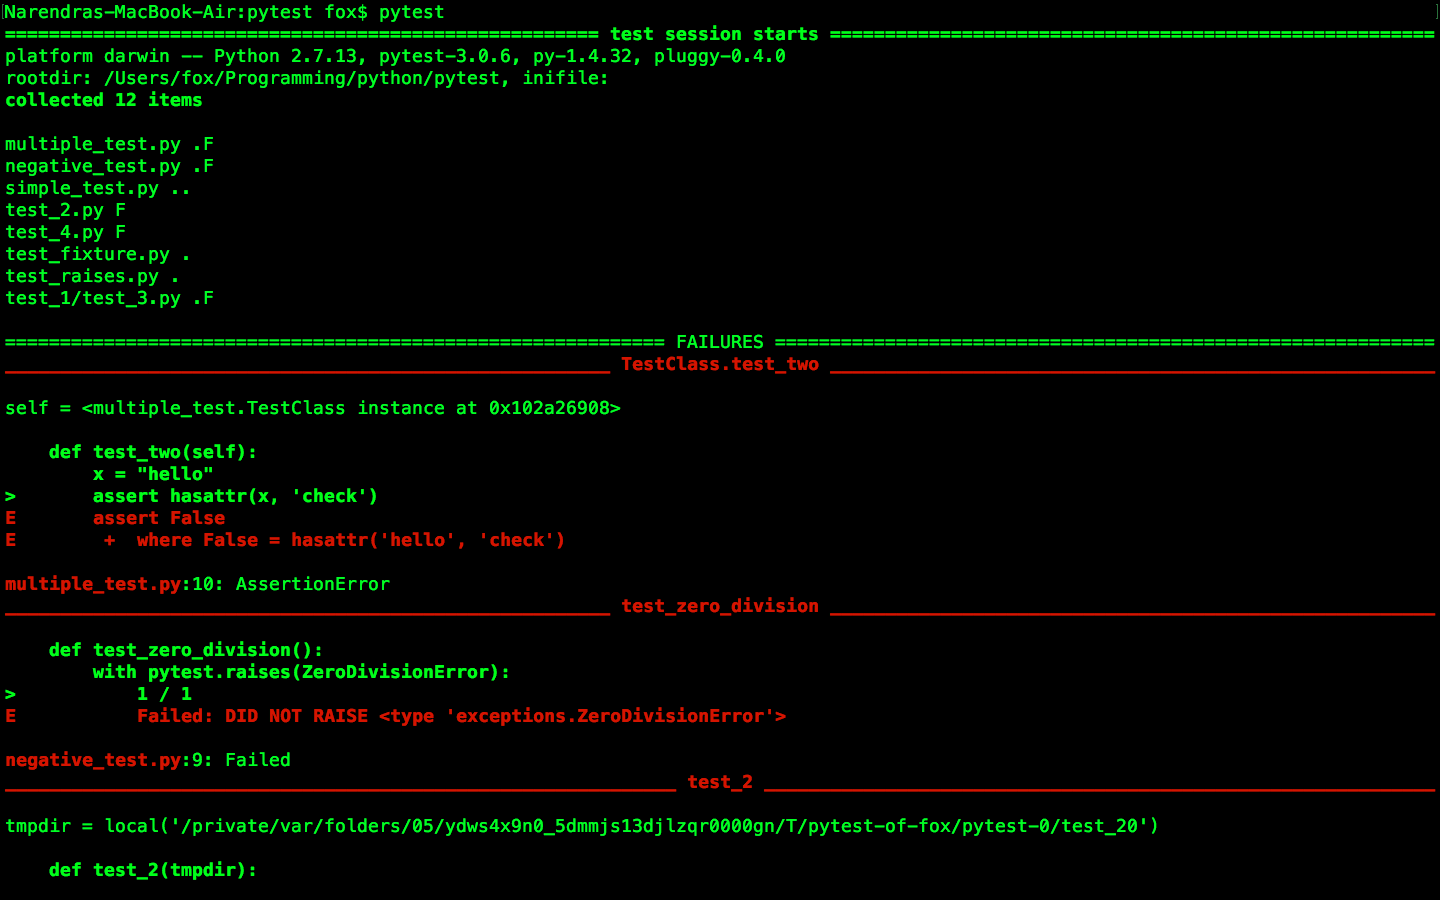
\includegraphics[width=\textwidth]{pytest}
    \caption{pytest for testing and debugging}
    \label{fig:5}
\end{figure}

\newpage
 % Introduction
\lhead{\emph{Chapter 2}}
\chapter{Implementation}

\section{Design}
The main objective of our project is to reduce the total number of writes. 

We have two approaches to achieve this. 
\begin{enumerate}

\item The first approach is by not replicating data to one of the replica, every time there is a write request from the client. The write is delayed for a fixed time and then initiated, this technique is called the \textbf{Lazy update.} 

\item The second is not replicating the data to any of the replicas instead log all the writes and then update the replicas after certain time. This avoids considerable program-erase cycles if same blocks are rewritten. We will call this \textbf{Logging.}

\end{enumerate}

With the first approach the replication is delayed to one of the replica nodes whereas with the second approach the delay is to all the replicas. Thus these approaches are more suitable for weak consistency applications. We wanted to design this approach on CEPH system. But due to time constraints and huge code base of CEPH we have gone ahead to design the model on a simple key, value based distributed system.

\begin{figure}[h]
    \centering
    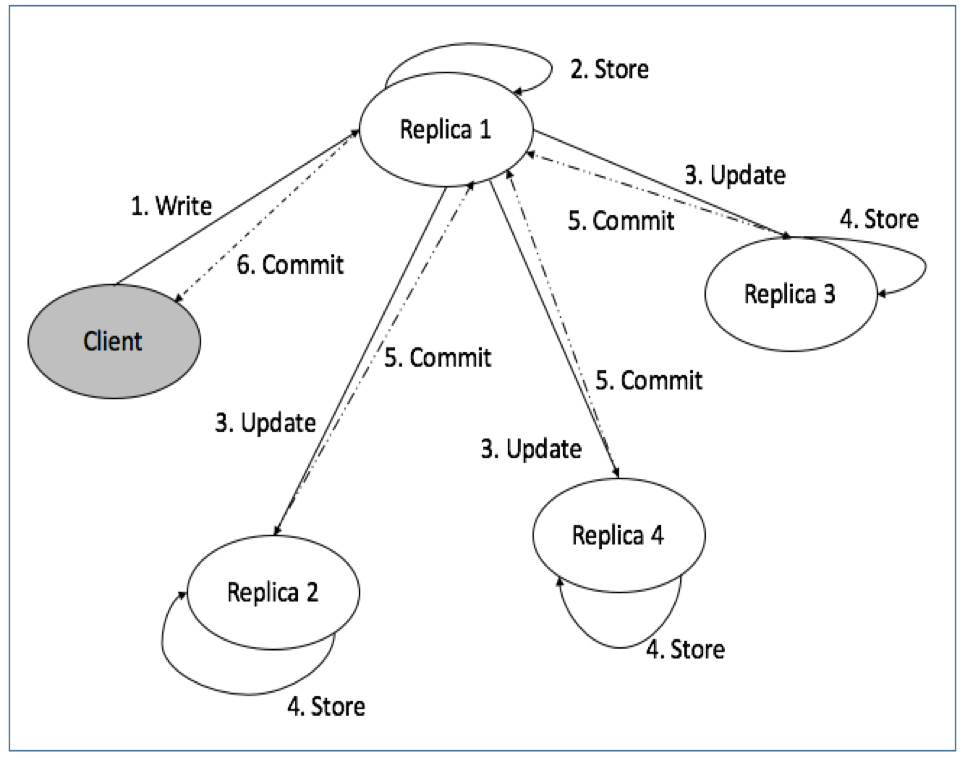
\includegraphics[width=\textwidth]{Figure1}
    \caption{Simple key, value pair Distributed System without our solution}
    \label{fig:21}
\end{figure}

Without our solution, the system would update the latest data immediately to all the replicas without any delay as shown in the figure \ref{fig:21}. Whenever there is a write request from the client, the data is replicated to all the replicas 1-4 immediately and simultaneously. This leads to more program-erase cycle thus lowering the endurance of the flash system.

\begin{figure}[h]
    \centering
    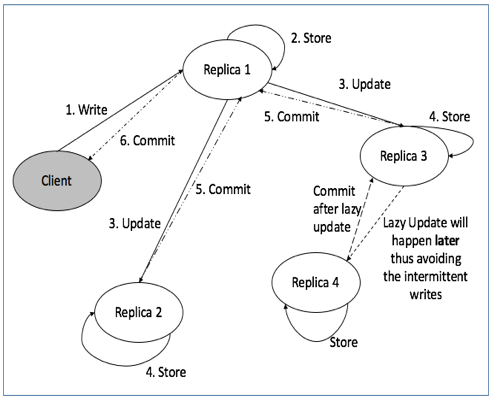
\includegraphics[width=\textwidth]{Figure2}
    \caption{Key, Value pair distributed system with lazy update on Replica 4}
    \label{fig:22}
\end{figure}

The data flow diagram with the first approach of our solution is as shown in the figure  \ref{fig:22}. 
A single replica is chosen from all the replicas for the lazy update. We have chosen Replica 4 for illustration purpose. On the event of a write request from the client, the data is replicated to all replicas immediately except for replica 4. Once all the other replicas store the new data and committed, the commit signal is sent back to the client. However, the update to replica 4 is delayed up to 2 minutes or until acceptable consistency delay. This way the number of writes to replica 4 is reduced. This increases the endurance of replica 4. With this approach, we will be able to improve the endurance of one node. The lazy update can be done to any one of the replicas for each write request on a round robin basis, thus improving endurance of all the nodes.


With the second approach, whenever a client sends a write request, it is logged in and commit signal is sent to the client. A finite number of writes is accumulated until it is actually written to all the replicas as shown in figure \ref{fig:23} below. After certain time, the accumulated writes are sent, all at once to all the replicas. This reduces the program-erase cycle of the flash system. With this approach, the intention is to improve the endurance of all the replicas.

\begin{figure}[h]
    \centering
    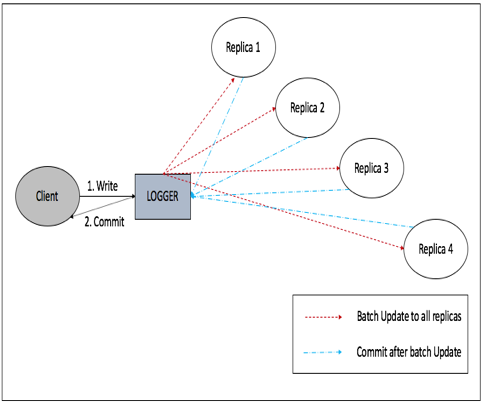
\includegraphics[width=\textwidth]{Figure3}
    \caption{Key, Value distributed system with logging for write events}
    \label{fig:23}
\end{figure}

\newpage

\section{File Structure}

The code is designed as Client Server model, where the server does the replication task and the client does the load generation. We have designed to support four instances of server code (replicas) running on different physical or virtual machine or at different network ports which is the \textbf{replicator.py} code. For the load generation we have clients running connected to different servers which is the \textbf{client.py} code. 

Apart from the above main code, the grapher.py code is used to plot the number of writes received from all the servers to get the dynamic write counts and to get the number of actual writes written from client which uses the writesfromclient.csv file.

For testing and debugging we have created the tox-quickstart and test cases files under the pytest folder. Pytest framework is used for testing. 

Refer figure \ref{fig:24} for file structure details. 

\begin{figure}[h]
    \centering
    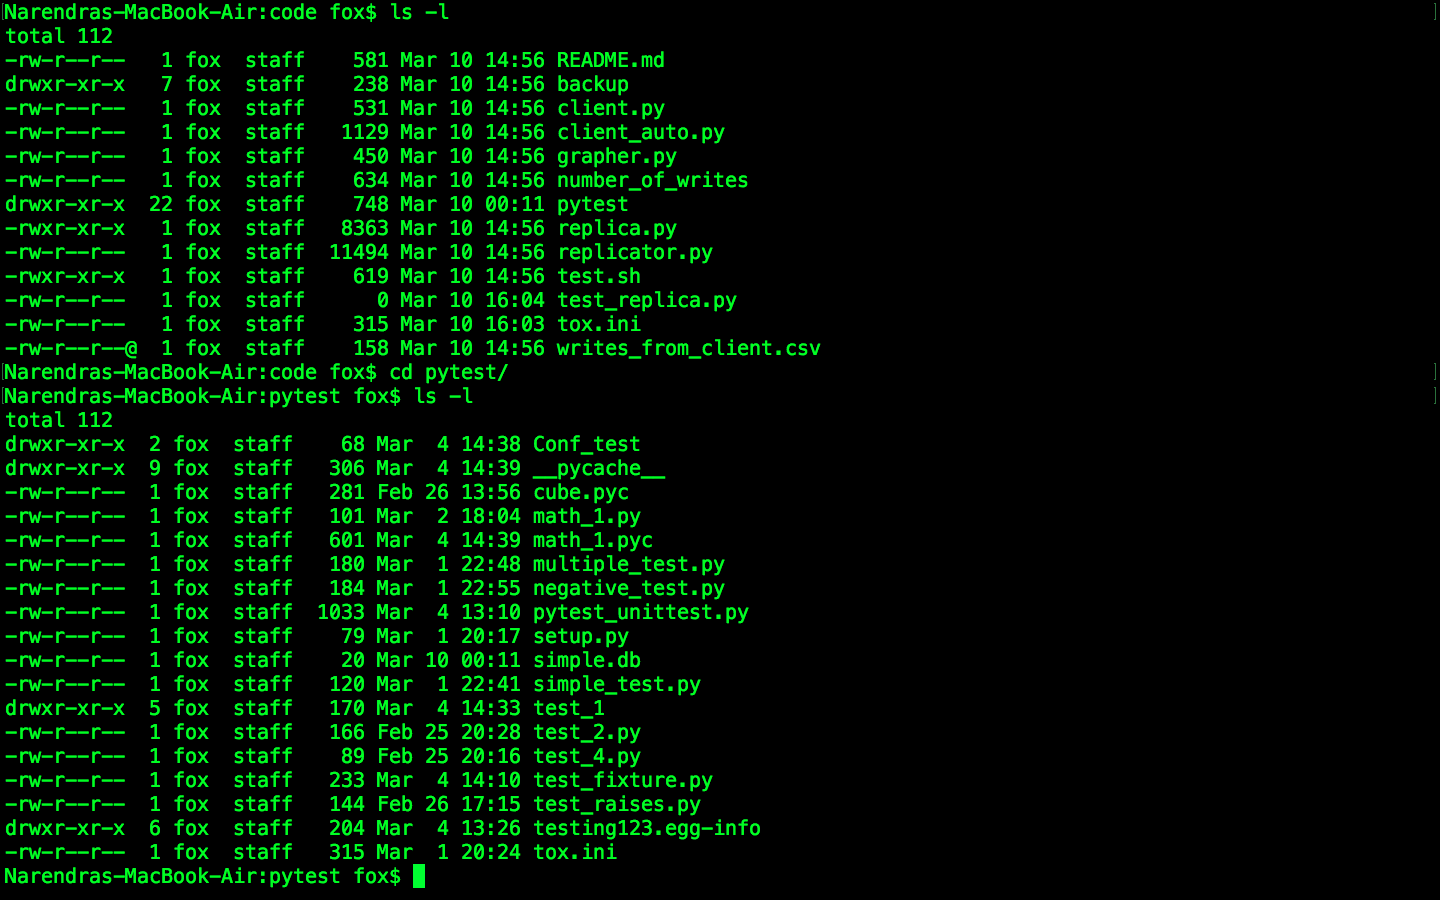
\includegraphics[width=\textwidth]{file_structure}
    \caption{File Structure}
    \label{fig:24}
\end{figure}

\section{Data Structures}

This Distributed system project is a type of dictionary data structure, where each key is unique and it stores a value. This data structure is replicated across all the disaster recovery sites using the network programming socket package which uses the TCP protocol. 

And again the same data structure which is the dictionary, is used to store the values at each of the sites. 

For this project we are using the pickledb package at each of the replicator and below are the commands supported by pickledb.

\textbf{\textit{DB operations available}}
\begin{enumerate}

\item  LOAD path dump  [Load a database from a file]

\item  SET key value [Set the string value of a key]

\item  GET key  [Get the value of a key] 

\item  GETALL [Return a list of all keys in database] 

\item  REM key [Delete a key] 

\item  APPEND key more [Add more to a key's value]

\item  LCREATE name [Create a list]

\item  LADD name value  [Add a value to a list]

\item  LGETALL name [Return all values in a list]

\item  LEXTEND name seq [Extend a list with a sequence]

\item  LGET name pos [Return one value in a list]

\item  LREM name [Remove a list and all of its values]

\item  LPOP name pos [Remove one value in a list]

\item  LLEN name [Return the length of a list]

\item  LAPPEND name pos more [Add more to a value in a list]

\item  DCREATE name [Create a dict]

\item  DADD name pair [Add a key-value pair to a dict, "pair" is a tuple]

\item  DGETALL name [Return all key-value pairs from a dict]

\item  DGET name key [Return the value for a key in a dict]

\item  DKEYS name [Return all the keys for a dict]

\item  DVALS name [Return all the values for a dict]

\item  DEXISTS name key [Determine if a key exists]

\item  DREM name [Remove a dict and all of its pairs]

\item  DPOP name key [Remove one key-value in a dict]

\item  DELDB [Delete everything from the database]

\item  DUMP [Save the database from memory to a file specified in LOAD]

\end{enumerate}

\section{Code Explanation}
It all starts by calling the python script replicator.py which will become the master replicator and the script will scan the ports and the mode of operation (Lazy update/Logging) provided by the user. 

The master replictor starts listening for the client`s connection request at the intiated port and parallely listens for all other slave replicators by using the hardcoded port numbers provided in the code. 

Later the user has to start other slave replicators on the TCP port which the master port is listening to. Thus establishing the connection between the master replicator and all the slave replicators. 

Next the client script should be started to make a connection to the master replicator. the client script is the load generator that will create the key value pairs. This generated load will be sent over the TCP socket created by the master replicator.

Once the master replicator receives the data from the client, it will be first copied to its local pickledb.  After few seconds the data will be written to the other slave replicas for disaster recovery or back up purpose. This mechanism is logging. 

Later to enhance the design, we added a mode called the lazy update which has the option for slave replicators to handle their own clients. If there is any update on the slave replicas as discussed above, data will be first written to the local pickledb and then it will be propogated to other slave nodes and the master node. But having the master node up all the time is a must, as it initiates the listening session for all the slave nodes. 

The initial design and implementation was done on a python disctionary later it was enhanced to support pickledb. Adding support for other data bases should be simple.

The difficulty was to debug the issues when we ran the code as we have distributed codes running in multiple sites.   inconsistent behaviour was seen while corelating any syncing up the multiple replication sites and clients to act as one system.  Triaging was very difficult while manual testing. To overcome this we automated the test cases and used  pytest for testing each function and debugging to see if we could achieve consistent behaviour. More about pytests and tox will be discussed later in Testing and Debugging section.

\newpage % Implementation
\lhead{\emph{Chapter 3}}
\chapter{Results}

\section{Overview}
As mentioned in the implementation we designed our own simple key value pair distributed data base, that supports simple DB commands and we have used the below two commands extensively. 

\textbf{\textit{DB Commands used extensively}}
\begin{enumerate}
\item SET 
\item GET
\end{enumerate}

 Once the data is sent by the client to any of the distributed system, instantly data will be replicated to all the available replicas. (Here for simplicity we have used 4 replicas). 

As the names of the commands represent we will be able to set a key with a value using the command: ``set 1 10``, that sets key 1 with value 10. And to retrieve the data we can execute the get command: ``get 1`` which fetches the value 10 in this example.

\section{Theoretical Analysis}
Theoretically the number of writes in a key value pair for a dictionary data structure will take 1 write for each value writes or update. In a replication setup the number of writes, will be equal to the number of replication sites times the number of writes. 

For analysis purpose lets consider we have 4 replication sites and for the regular key-value pair data structure, we will have 4 times the number of key-value update. Which is depicted in the graph \ref{fig:8}.

\begin{figure}[!htbp]
    \centering
    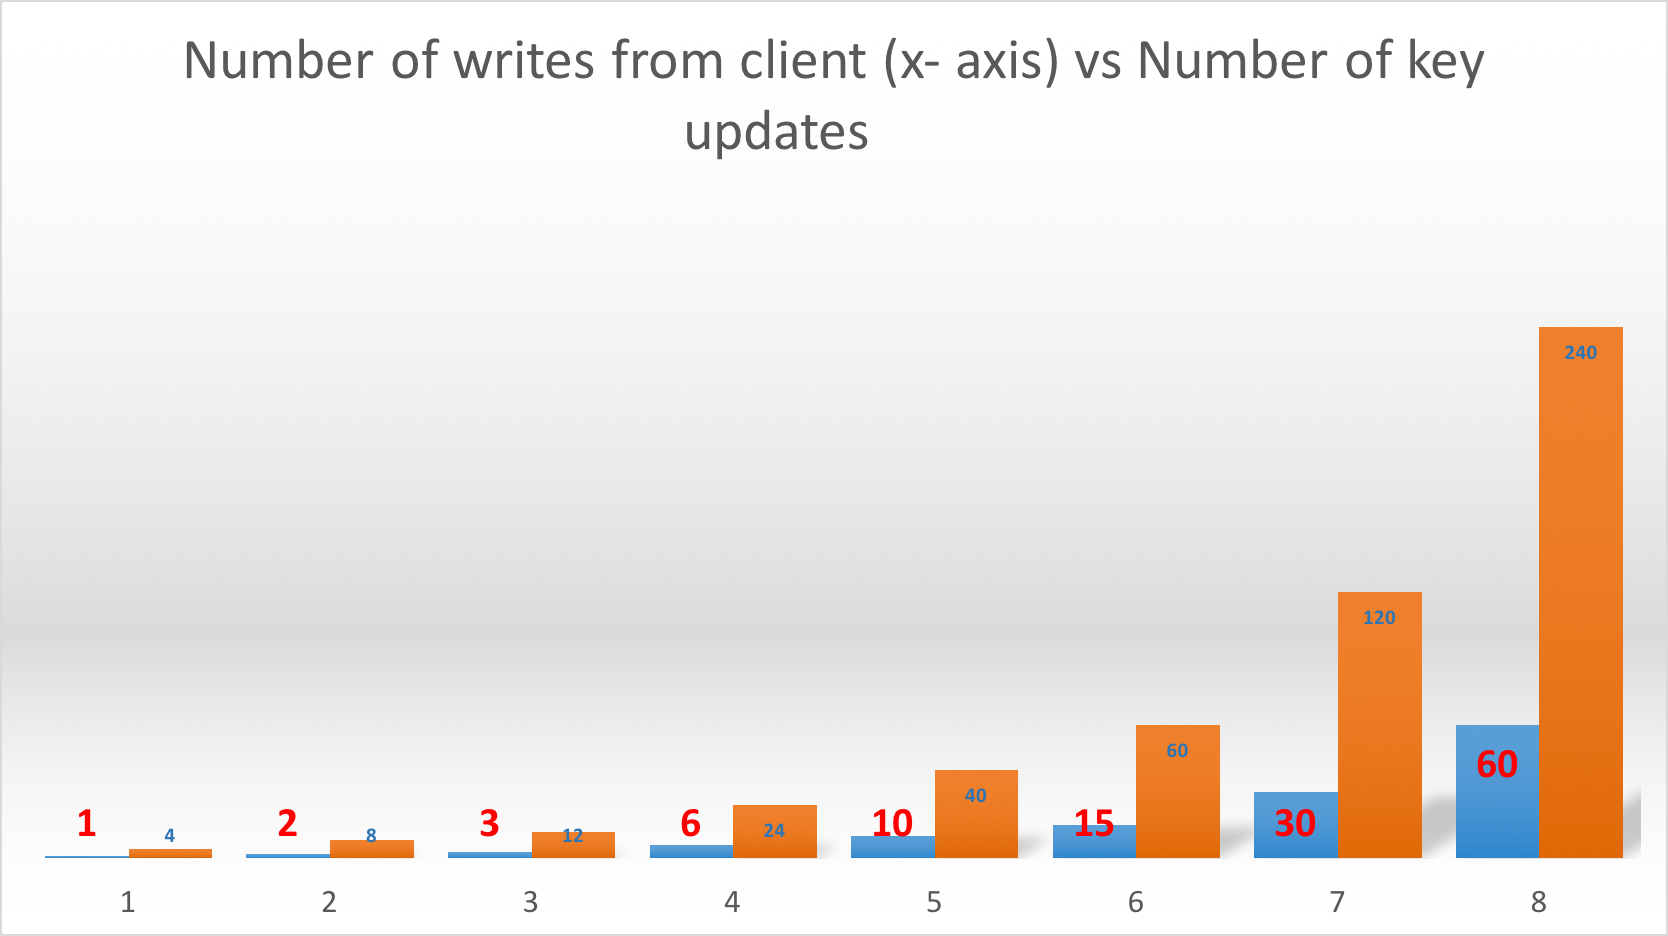
\includegraphics[width=\textwidth]{Plot1}
    \caption{ Theoretical estimate for simple key, value pair distributed system without our solution.}
    \label{fig:8}
\end{figure}

\begin{figure}[!htbp]
    \centering
    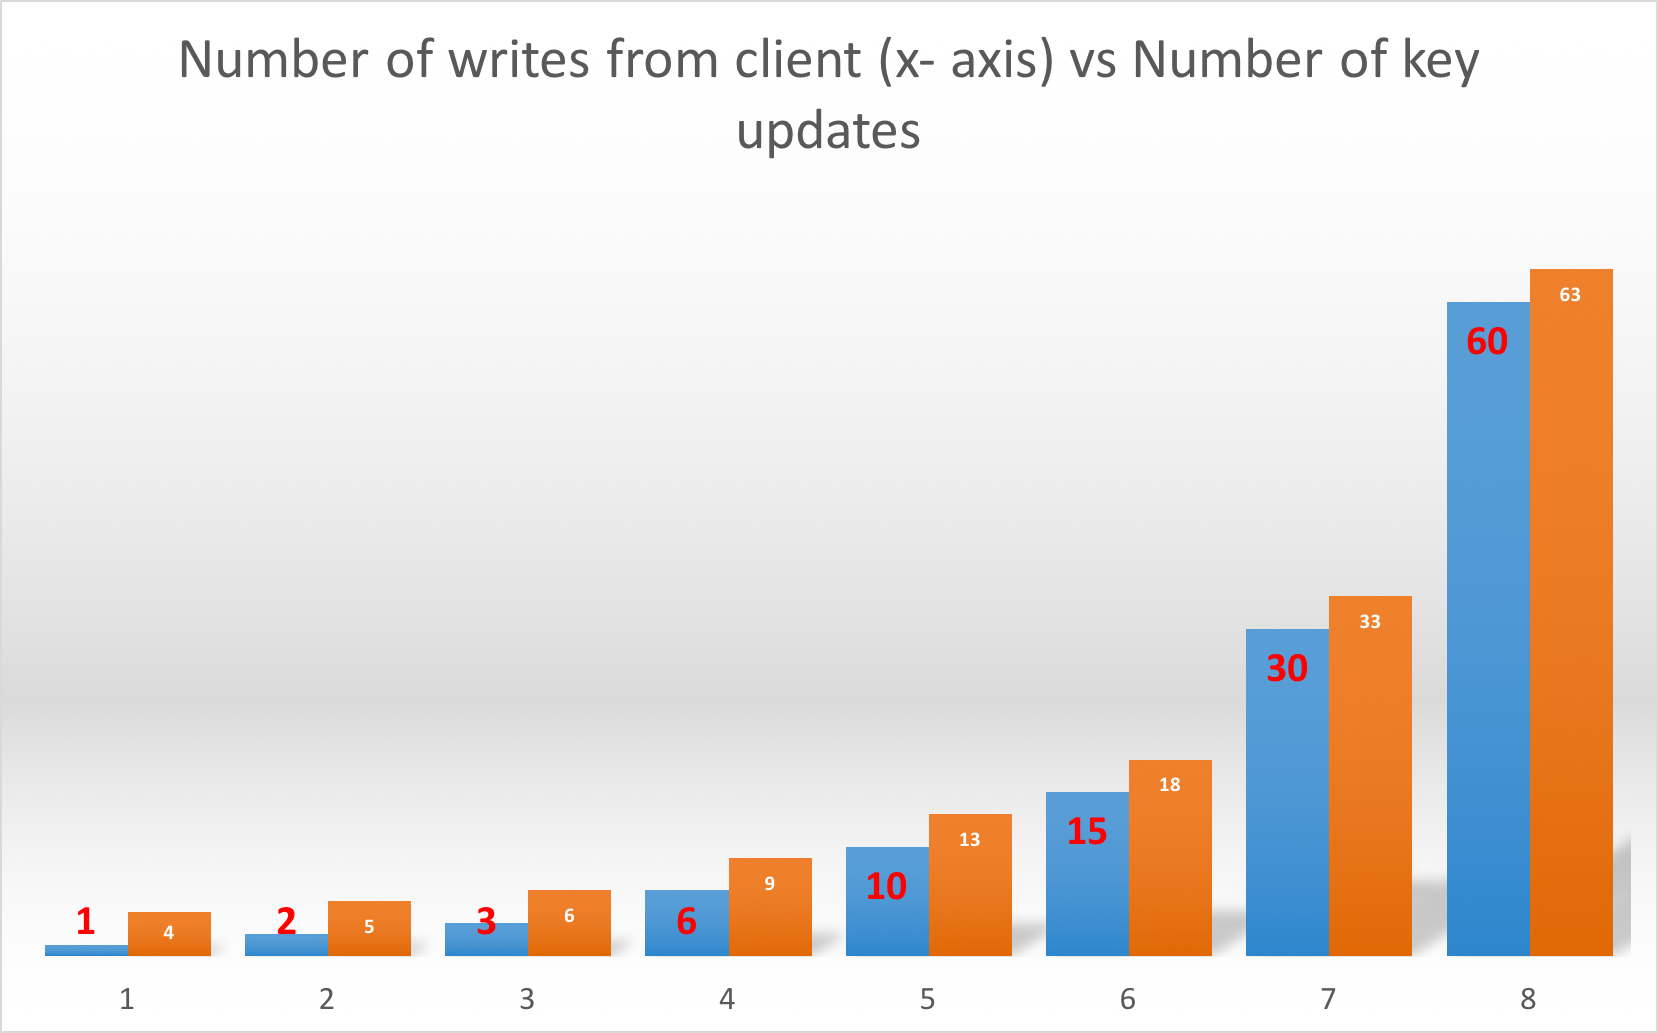
\includegraphics[width=\textwidth]{Plot2}
    \caption{Theoretical estimate for simple key, value pair distributed system with our solution of logging.}
    \label{fig:9}
\end{figure}

Similarly for theoretical analysis lets consider we have the logging mechanism where we have same 4 replication sites. Instead of writing all the writes immediately, the writes are delayed and replicated after 30 seconds. So theoritcally we will be writing only once for each of the key-value update until 30 seconds. Lets assume we will have around 60 writes during 30 seconds, in this scenario there will be only 60 writes to the main replicator and plus 3 for other replictors, which totalls to 63 writes instead of 240 writes. Here we are assuming that we will have 60 update to the same key-value. So we are saving {240 - 63 = 177} writes.

%Once the data is available at one of the replicas instead instantly sending the updates to all the replicas we will accumulated the writes in the log we will wait for 30 second timer and later update the data to all the replicas, by this we were able to save approximately 20 key updates to 3 of the replicas, so we were able to save 60 writes to the flash storage. After 20 key updates our 30 second timer was done and we have to send all the writes accumulated so when we had the 30 key updates we updated all the accumulated key writes to all the replicas. So we are seeing that 120 key update in our solution too in figure 5.



%\newpage
\section{Practical Results}

To implement logging solution as discussed in implementation, we created a timer mechanism in which captured all the writes in the log and wait for specified interval of time say 30 seconds. (This can be tuned as per the requirement and for the remainder of the example we will consider timer of 30 seconds.)
%\begin{figure}[!htbp]
 %   \centering
 %   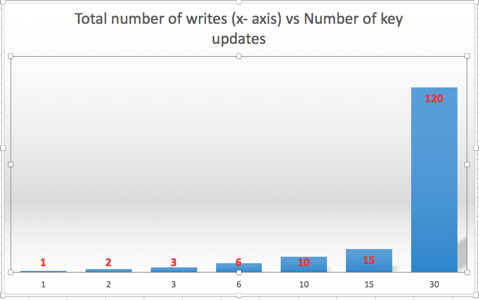
\includegraphics[width=\textwidth]{Figure5}
  %  \caption{Graph for simple key, value pair distributed system with our solution of logging.}
%    \label{fig:9}
%\end{figure}

Practically with our solution we were able to observe the below comparison and there is difference in the theoretical and the practical values. This is because we are using a random number gnerator for load generation and also the timer will not be synced with all the 4 sites.

Figure \ref{fig:10} and \ref{fig:11} are the comparison of total number of writes actually generated at the clients to the total number of writes done at the replicas without and with our solution respectively.

\begin{figure}[!htbp]
    \centering
    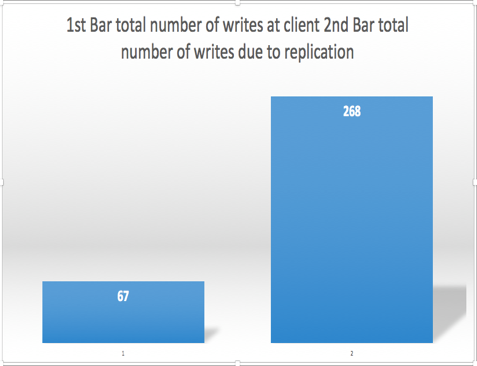
\includegraphics[width=\textwidth]{Figure6}
    \caption{Practical results: Total number of writes from all the clients against the total number of key value updates across replicas without our solution.}
    \label{fig:10}
\end{figure}


The total number of writes for 67 updates with out our solution were 268 writes. Whereas with our solution the number of writes at all the replicas totalled to 157 for the same 67 updates from the client. We can see from this that we were able to save a total of 111 writes, so there was a reduction of 58 percent of writes.

\begin{figure}[!htbp]
    \centering
    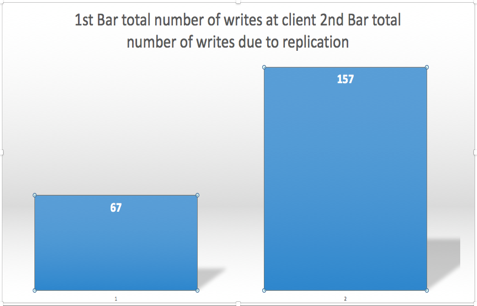
\includegraphics[width=\textwidth]{Figure7}
    \caption{Practical results: Total number of writes from all clients against the total number of key value updates across replicas using the logging solution.}
    \label{fig:11}
\end{figure}

Complete project code is available under: \href{https://github.com/Narendrakumarg1728/write_reduction_in_Distributed_replicas}{GIT HUB link}

\newpage % Testing
\lhead{\emph{Chapter 4}}
\chapter{Debugging and Testing}

In order to test and debug, ``pytest'' needs to be installed. Once it is installed, it is as simple as calling the pytest with the executable script to run and verify the results. 

\textbf{\textit{Brief description of pytest}}

 It is a test framework written in python to test code written in python.

Very easy to start using the framework and supports to scale complex functional testing.

Community support and documentation is very good.

Supports 150+ plugins.



For our project we used below functionalities which is available in python and part of pytest for tetsing and debugging.

\begin{enumerate}
    \item assertion  [For testing each function, works like "if not" and raises an exception]
    \item fixtures  [For setting up configuration before and then to do clean up after testing is completed] 
    \item pytest.raises [To perform negative testing and to test exceptions] 
    \item conftest [Used to provide the config details and to provide scope of the fixtures]
    \item tox [To create virtual enviranment which provides option to select different verisons of the packages and python versions]
    \item devpi[Repository manager]
\end{enumerate}

The figure \ref{fig:14} displays all the above operation done in python.


\newpage

\begin{figure}[h]
    \centering
    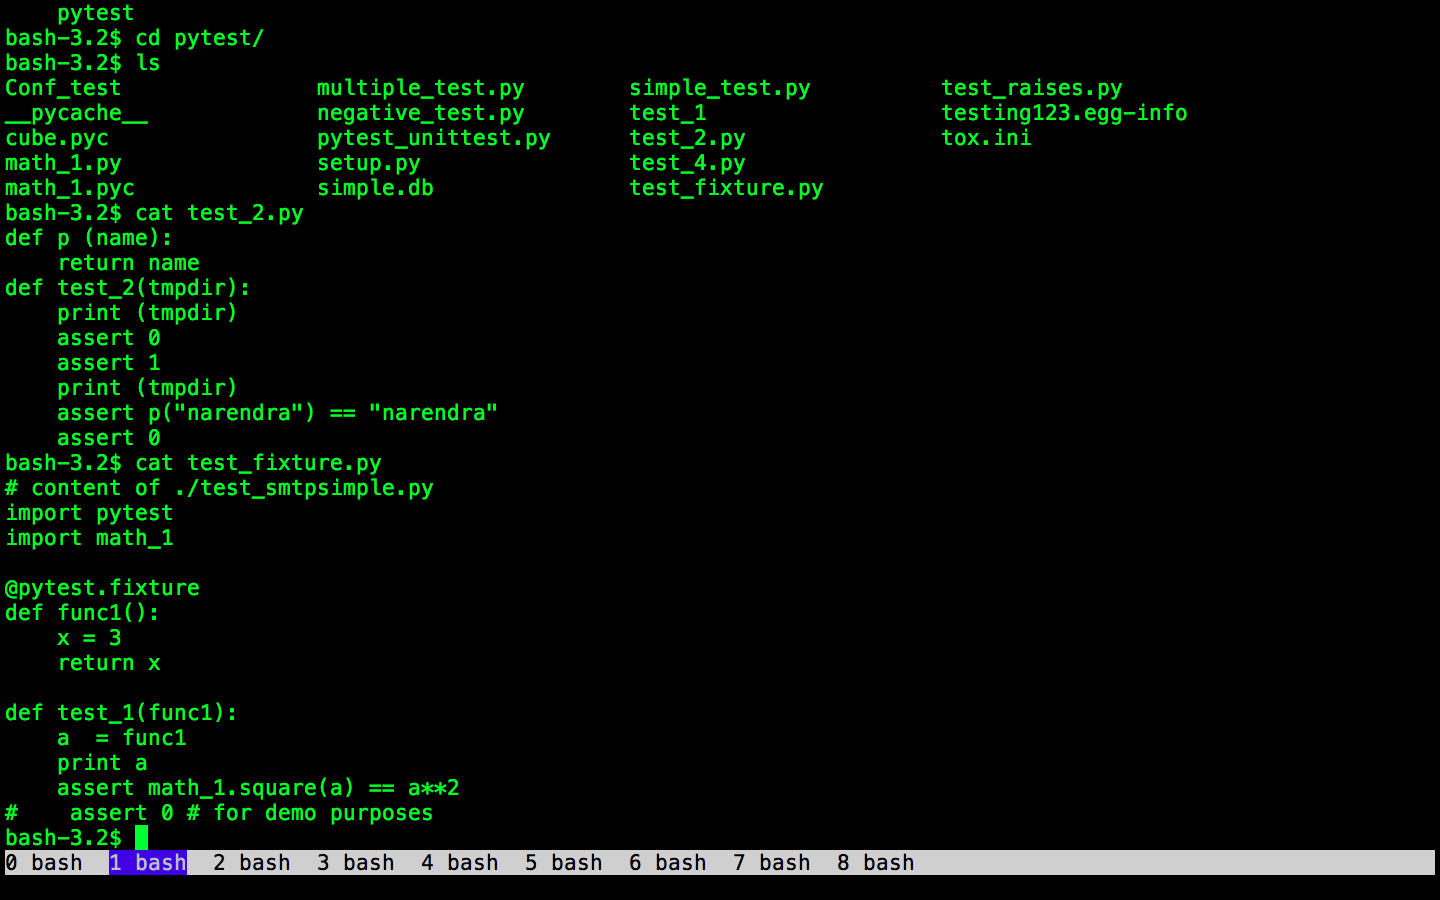
\includegraphics[width=\textwidth]{pytest2}
    \caption{Testing and Debugging in pytest}
    \label{fig:14}
\end{figure}

\newpage % Debugging
\lhead{\emph{Chapter 5}}
\chapter{Improvements}
%The main idea of this project is to build a software to support reduction of the data writes on a flash drives by writing the data only on few of the copies if the same copy exixtis in multiple places. To illustrate this as a proof of concept  we have choosen the distributed system scenario where we have multiple copies of same data in multiple disaster recovery sites. 
The main idea of the project was to explore memory and storage coordinative ECC and wear leveling schemes across memory and storage components to implement a solution where the number of writes on the disk can be reduced as we have the same data on the RAM. 

This requires access to SSD firmware and the OS driver which are proprietary softwares. It is difficult to get access and requires high technical knowledge to understand and implement the firmware code which also requires lots of time effort. 

Our project is the proof of concept to show that we can have write reduction and this should be extended to support for the SSD drives in the future.

\textbf{Other features which can be extended for this project are:}
\begin{itemize}
    \item Support general data bases like SQL DB.
    \item Use data from real scenario for data generation.
    \item Integrate IO-meter as the data generator. 
\end{itemize}
\newpage % Improvements
\lhead{\emph{}}
\textbf{\textit{References}}
\begin{enumerate}

\item  {RELIABLY ERASING DATA FROM FLASH-BASED SOLID STATE DRIVES: Michael Wei, Laura M. Grupp, Frederick E. Spada  , Steven Swanson University of California, San Diego}

\item {STUDY OF BAD BLOCK MANAGEMENT AND WEAR LEVELING IN NAND FLASH MEMORIES: Supriya Kulkarni P1, Jisha, Electronics and Communication Dept, MVJ Engineering, Bangalore}

\item  {HRAID6ML: A HYBRID RAID6 STORAGE ARCHITECTURE WITH MIRRORED LOGGING: Lingfang Zeng, Dan Feng , Janxi Chen  Qingsong Wei, Bharadwaj Veeravalli , Wenguo Liu}

\item  CSWL: CROSS-SSD WEAR-LEVELLING METHOD IN SSD-BASED RAID SYSTEMS FOR SYSTEM ENDURANCE AND  PERFORMANCE: Kwanghee Park, Dong-Hwan Lee, Youngjoo Woo, Geunhyung Lee, Ju-Hong Lee, Deok-Hwan Kim Dept. of Electronic Engineering, Inha University.

\item  RELAIBILITY AND PERFORMANCE ENHANCEMENT TECHNIQUE FOR SSD ARRAY STORAGE SYSTEM USING RAID MECHANISM: Kwanghee Park, Dong-Hwan Lee, Youngjoo Woo, Geunhyung Lee, Ju-Hong Lee, Deok-Hwan Kim Dept. of Electronic Engineering, Inha University.

\item  AN EMBEDDED FTL FOR SSD RAID: Alistair A. McEwan and Irfan Mir Department o f Engineering University of Leicester, Leicester LE1 7RH, UK

\item  RELIABILITY MANAGMENET TECHNIQUES IN SSD STORAGE SYSTEMS : Irfan F. Mir University of Leicester 

\item BUILDING FLEXIBLE, FAULT TOLERANT FLASH BASED STORAGE SYSTEMS: Kevin M. Greenan Darrell D.E. Long Ethan L. Miller  Thomas J. E. Schwarz, S.J.  Avani Wildani  Univ. of California, Santa Cruz  Santa Clara University 

\item WEAR LEVELLING USING MACHINE LEARNING: Coughlin Associates, Flash Memory Summit 2016.

\item REJUVENATOR: A STATIC WEAR LEVELLING ALGORITHM FOR FLASH MEMORY: Murugan.M, Du. D, Department of Computer Science, University of Minnesota

\item INCITS Technical Committee T10 TRIM command RFEs

\item Image \ref{fig:1} from \href{http://hyperphysics.phy-astr.gsu.edu/hbase/quantum/barr.html}{hyperphysics} 

\item Image \ref{fig:2} from \href {https://www.fhwa.dot.gov/publications/research/infrastructure/pavements/12072/002.cfm}{fhwa.gov}  

\end{enumerate}
 % References

%% -------------------------------------------------------

\end{document}